\section{RELATED WORKS}
\label{sec:related_works}

The estimation of additional fuel consumption arising from air traffic management operations has emerged as an important research topic due to its operational, economic, and environmental implications. The growing availability of operational data and advances in machine learning techniques have driven the development of increasingly accurate methods for modeling fuel consumption and atmospheric emissions.

\subsection{ATM Performance Indicators}
In the context of the performance-based management advocated by the International Civil Aviation Organization (ICAO), Key Performance Indicators (KPIs) are essential metrics used to quantitatively express past and current operational performance against organizational objectives. In the aviation industry, KPIs are crucial for enhancing governance and operational efficiency in a highly complex and regulated sector. By relying on standardized metrics, stakeholders can identify bottlenecks, measure outcomes, and promote continuous improvements in safety, punctuality, airport capacity, and environmental sustainability.

Furthermore, the systematic analysis of KPIs facilitates communication among airport operators, airlines, air navigation service providers (ANSPs), and regulatory bodies, fostering a shared vision of strategic goals. KPIs also play a vital role in aligning aviation operations with international policies, such as the United Nations Sustainable Development Goals, by measuring environmental impacts like fuel consumption and emissions.

In this study, two specific performance indicators established by ICAO are of primary interest: KPI08: Additional Time in TMA, and KPI16: Additional Fuel Burn. Both metrics combined are essential to evaluate aircraft performance at Terminal Maneuvering Area (TMA) in terms of time, fuel consumption and emissions. However, this work focuses on the development of predictive models for KPI16, as predicting additional fuel burn is crucial for understanding and mitigating environmental impacts, as well as providing companies and air traffic managers actionable insights to optimize operations and reduce costs.

\subsubsection{KPI08: Additional Time in TMA}
KPI08 measures the additional transit time spent by an aircraft within the TMA compared to an unimpeded baseline, considered as the optimal transit time. In this study, the Terminal Area is defined as a cylindrical airspace with a 100-nautical-mile radius centered at Guarulhos (GRU) International Airport. The reference baseline is generally established through the clustering of transit time samples based on the runway in use, the aircraft type, and the entry sector into the terminal area. As illustrated in Figure \ref{fig:gru_sectors}, these entry sectors are divided into angular segments of 60 degrees. The unimpeded transit time is then defined as the 20th percentile of all samples within these grouped conditions. According to the MCA 100-22 methodology \cite{mca10022}, this 20th percentile threshold was established following ICAO recommendations, which identified that, statistically, the 20th percentile ($P_{20}$) provides a robust approximation of an unimpeded reference value. Additionally, this selection inherently incorporates a treatment for outliers in the operational dataset.

\begin{figure}[htbp]
    \centering
    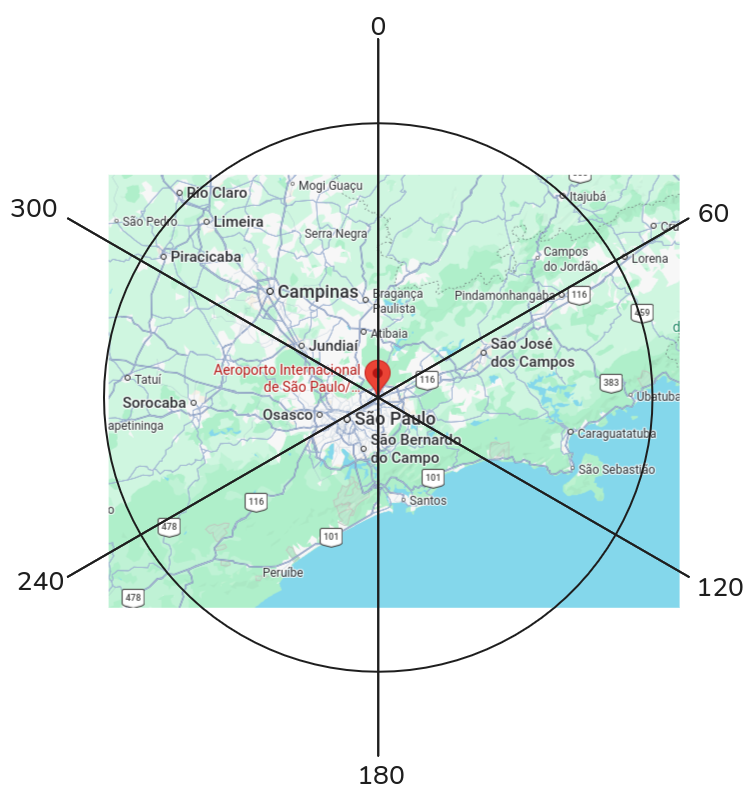
\includegraphics[width=0.8\linewidth]{images/gru_sectors.png}
    \caption{Guarulhos International Airport (GRU) Terminal Maneuvering Area (TMA) and its 60-degree entry sectors.}
    \label{fig:gru_sectors}
\end{figure}

Various factors can influence this indicator, including airspace design, meteorological conditions, and tactical interventions by Air Traffic Control (ATC) such as holding patterns and vectoring for sequencing. The comparison of the actual transit time to the 20th percentile baseline effectively isolates the operational inefficiencies, focusing on the ATM's responsibility in optimizing the arrival flow.

\subsubsection{KPI16: Additional Fuel Burn}
KPI16 represents the core metric for evaluating ATM-induced operational efficiency from an environmental perspective, providing an aggregate view of the excess fuel consumed during a flight phase. In the context of TMA operations, it is directly correlated with the inefficiencies captured by KPI08.

There are various methods for calculating KPI16. In Brazil, the Department of Air Space Control (DECEA) adopts a strategy similar to KPI08, as the additional fuel burn is calculated as the difference between the actual fuel consumed by an aircraft and a reference fuel consumption. Like KPI08, this baseline is determined as the 20th percentile of fuel consumption for similar flights. Positive values of KPI16 indicate fuel consumption above the expected optimal level—often resulting from airspace congestion and ATC interventions—whereas negative values indicate flights that operated more efficiently than the established baseline. As the target variable of the predictive models developed in this work, KPI16 serves as a direct proxy for the environmental and economic cost of ATM inefficiencies in the terminal area.

In this context, a shift can be observed from traditional approaches based on physico-mathematical models towards data-driven methodologies. Broadly, the literature can be organized into three main research streams: (i) aircraft performance modeling, (ii) operational analysis of Air Traffic Management (ATM), and (iii) the application of machine learning for fuel consumption and emissions estimation.

\subsection{Aircraft Performance Modeling}
The first research stream focuses on aircraft performance modeling. The Base of Aircraft Data (BADA) model, developed by EUROCONTROL \cite{nuic2010bada}, has become one of the primary references for aircraft performance studies, flight planning, trajectory simulation, and environmental assessments, providing widely used parametric performance models for ATM research. Subsequently, Del Pozo \textit{et al.} \cite{delpozo2022bada} proposed calibrating BADA coefficients using machine learning techniques and operational flight data, reducing discrepancies between nominal and observed in-service performance.

More recently, Jarry \textit{et al.} \cite{jarry2024generalization} investigated deep learning models for fuel flow estimation capable of generalizing across different aircraft types, while Jarry \textit{et al.} \cite{jarry2025ageing} incorporated engine ageing effects into fuel consumption modeling using Quick Access Recorder (QAR) data. In a similar vein, architectures based on Multi-Layer Perceptrons (MLP), Radial Basis Functions (RBF), and Recurrent Neural Networks (RNN) have been employed to develop tail-specific models \cite{hetherington2025tail}, exploiting QAR data to represent individual degradation and operational patterns.

Although these approaches achieve high accuracy in estimating fuel consumption, their application depends on high-frequency proprietary QAR data, which is typically unavailable to Air Navigation Service Providers (ANSPs). Furthermore, these models are primarily designed to represent the physical performance of individual aircraft rather than to estimate the operational fuel penalties arising from ATM inefficiencies. This limitation reduces their scalability and hinders their adoption in operational applications that rely exclusively on surveillance data and information routinely available to ANSPs.

\subsection{ATM Operational Analysis}
The second research stream investigates ATM operational efficiency. Kwasiborska and Skorupski \cite{kwasiborska2021merging} analyzed the environmental impact of different aircraft stream merging strategies during the approach phase, demonstrating that traffic flow organization directly influences additional flight time and, consequently, fuel consumption. In a complementary approach, Krauth \textit{et al.} \cite{krauth2023generative} developed a generative model based on Variational Autoencoders (VAEs) to generate realistic four-dimensional trajectories in Terminal Maneuvering Areas (TMAs), accounting for uncertainties arising from ATC interventions, meteorological conditions, and aircraft performance variability.

Although these studies contribute significantly to the understanding of air traffic dynamics and trajectory variability, their primary focus lies in trajectory simulation, operational flow analysis, and ATM scenario evaluation, rather than in the direct estimation of fuel penalties associated with ATM operational inefficiencies.

\subsection{Machine Learning for Fuel Consumption and Emissions Estimation}
A third research stream applies machine learning techniques to the estimation of fuel consumption and atmospheric emissions. Al Kazzaz \cite{alkazzaz2025emissions} developed an Artificial Neural Network (ANN) trained on data from the ICAO Engine Emissions Databank (EEDB) to predict fuel consumption and CO\textsubscript{2}, NO\textsubscript{x}, and CO emissions using engine parameters, fuel properties, and operational conditions. The study demonstrated that integrating ADS-B data, meteorological conditions, and engine characteristics can improve in-flight emission estimation. However, these studies concentrate on estimating aircraft atmospheric emissions rather than on quantifying the operational fuel penalties arising from ATM inefficiencies.

\subsection{Research Gap and Contribution}
Despite the advances observed across these research streams, an important gap remains in the literature. Existing studies focus predominantly on detailed aircraft performance modeling using proprietary on-board data such as QAR, on trajectory simulation, or on atmospheric emissions estimation. By contrast, few studies directly investigate the additional fuel consumption arising from ATM operational inefficiencies using exclusively operational data routinely available to ANSPs.

In this context, the present work proposes a machine learning–based approach to estimate Key Performance Indicator 16 (KPI16) using radar surveillance data, BADA performance parameters \cite{nuic2010bada}, ATM operational indicators, and meteorological information available prior to or at the moment of TMA entry. In contrast to Jarry \textit{et al.} \cite{jarry2024generalization, jarry2025ageing}, who focus on fuel flow modeling from high-fidelity QAR data; Krauth \textit{et al.} \cite{krauth2023generative}, whose focus lies in four-dimensional trajectory generation through generative models; and Al Kazzaz \cite{alkazzaz2025emissions}, whose work targets atmospheric emissions estimation, this study concentrates on predicting the additional fuel consumption associated with ATM operational inefficiencies. By integrating data sources routinely available to ANSPs, the proposed methodology advances the state of the art by enabling scalable KPI16 estimation applicable to the continuous monitoring of operational efficiency and environmental performance in terminal areas.
